\documentclass[../main.tex]{subfiles}

\begin{document}
\section{Methods}
\subsection{Stimulus Generation}
We used GANalyze with AestheticsNet \parencite{kongPhotoAestheticsRanking2016} as the discriminator and BigGAN-256 \parencite{brockLargeScaleGAN2019} pretrained on ImageNet \parencite{russakovskyImageNetLargeScale2015} as the generator to train the GANalyze model for 400,000 iterations. To do this, we used Python 3.6 with the \texttt{TensorFlow} libraries \parencite{abadi2016tensorflow}. The training resulted in GANalyze being able to produce image sequences based on 1,000 ImageNet categories. For each ImageNet category, we initially generated three different seeds (e.g., three different images of Siamese cats) to test for an effect of idiosyncratic effects of images on top of semantic category. Within each seed, GANalyze produced 21 images with a supposedly increasing amount of aesthetic value (Figure ~\ref{fig:sample_sequence}). We picked a broad range of $\alpha$-values with increasing density close to zero to obtain stimuli with obvious changes (e.g., $\alpha$ = 0.25), but also subtle changes (e.g., $\alpha$ = 0.0025). We chose these values because we hypothesized there to be a ceiling effect where there would be no behavioral differences for extremely high $\alpha$-values due to oversaturation. We also hypothesized that for very low $\alpha$-values, the perceptual difference between stimuli would be too small to detect. The specific $\alpha$-values used in the final experiment were chosen based on the results of a pilot study with a wider variety of $\alpha$'s. This pilot followed the same general structure as the full experiment which is explained below. The main difference in the pilot is the use of the unfiltered dataset with 21 $\alpha$-values and 3 seeds. This pilot showed us that we would be justified to only use one of the three seeds for each category. More details about this pilot study are reported in the Results section.

\begin{figure}[!h]
	\caption{Sample of an Image Sequence With Five $\alpha$-values}
	\label{fig:sample_sequence}
	\centering
	\begin{subfigure}{.18\textwidth}
		\centering
		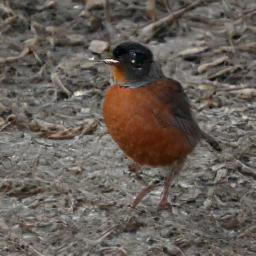
\includegraphics[width=1\linewidth]{methods/1}
		\caption{\centering $\alpha = -0.25$}
	\end{subfigure} \hfill
	\begin{subfigure}{.18\textwidth}
		\centering
		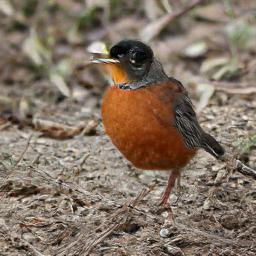
\includegraphics[width=1\linewidth]{methods/2}
		\caption{\centering $\alpha = -0.10$}
	\end{subfigure} \hfill
	\begin{subfigure}{.18\textwidth}
		\centering
		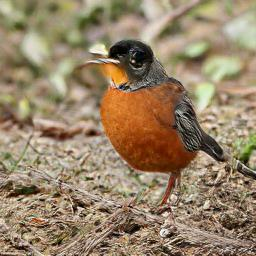
\includegraphics[width=1\linewidth]{methods/3}
		\caption{\centering $\alpha = 0$}
	\end{subfigure} \hfill
	\begin{subfigure}{.18\textwidth}
		\centering
		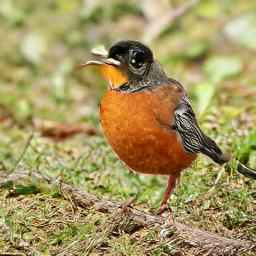
\includegraphics[width=1\linewidth]{methods/4}
		\caption{\centering $\alpha = 0.10$}
	\end{subfigure} \hfill
	\begin{subfigure}{.18\textwidth}
		\centering
		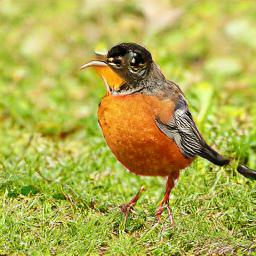
\includegraphics[width=1\linewidth]{methods/5}
		\caption{\centering $\alpha = 0.25$}
	\end{subfigure} \hfill
\end{figure}

511 ImageNet categories were manually excluded from the stimulus set because they either contained human faces (which are deliberately warped by BigGAN), insects such as spiders which might make some participants feel uncomfortable, or for redundancy such as the disproportionately high number of categories about dog breeds. In addition, stimuli that we considered to be unrecognizable were also excluded. This resulted in 489 categories, each with one seed and 15 $\alpha$-values, equaling a total of 7,335 stimuli. We grouped the ImageNet categories in 8 broader groups based on their content. The groups we created are `animal', `clothing', `food', `indoor', `nature', `outdoor', `tool', and `vehicle'. These groups were only used to test for an effect of semantic content.
	

	
\subsection{Questionnaire}
To measure the aesthetic experience of each participant, we used a shortened version of the Aesthetic Experience Questionnaire \parencite[AEQ;][]{wanzerExperiencingFlowViewing2020}. We have chosen this particular questionnaire based on a number of factors. First of all, the theoretical background of an aesthetic flow experience \parencite{csikszentmihalyi1990art} is valid under our assumed interactionist conception of beauty. Second, this questionnaire seems fitting because the AEQ is designed to be generalizable to all visual aesthetic experiences and is not limited to famous pieces in a museum as is the case with many other questionnaires. Finally, we picked the AEQ because the authors suggest that it should be possible to reduce the items on the six scales and still end up with a sufficient measurement of aesthetic experience.

As the experience one has with art was not the primary focus of our study, we only used the highest loading items from each of the six scales, resulting in a total of six items at the start of our study in order to save time (see Appendix A). Each item was presented with a five-point Likert scale, ranging from 0 (\textit{Strongly disagree}) to 4 (\textit{Strongly agree}). To test whether this shortened version of the AEQ was sufficient to explain the latent aesthetic experience, we used confirmatory factor analysis (CFA).
	
	
	
\subsection{Behavioral Experiment}
To determine whether GANalyze can be used to study what it means for an image to be aesthetic, we conducted a behavioral study to test whether human participants indeed preferred the images that GANalyze generated to be more aesthetic over a corresponding base image. This study has been approved by the Social and Societal Ethics Committee of the KU Leuven (SMEC).
	
The study was hosted on Prolific.co to obtain a large number of data points in a simple online task, ensuring each of the 7,335 stimuli was evaluated around 20 times on average. Individuals younger than 17 or those without normal or corrected-to-normal vision were not allowed to participate. Task instructions were provided on the main Prolific of this experiment and had to be read before starting the experiment (see Appendix B). The online experiment started with an informed consent document which had to be signed, followed the AEQ. After the AEQ, the main task was initiated. The participants carried out a spatial two-alternatives forced choice (2AFC) task in which they had to indicate which of the two presented GAN-generated images they considered to be most aesthetically pleasing. They did this by pressing "F" for the left, and "J" for the right image (Figure~\ref{fig:trial_sequence}). Participants were instructed that because there was no real correct answer, they should only select the image they personally preferred.

\begin{figure}[!h]
	\begin{center}
		\caption{Example of a Sequence of Trials in the Study}
		\label{fig:trial_sequence}
		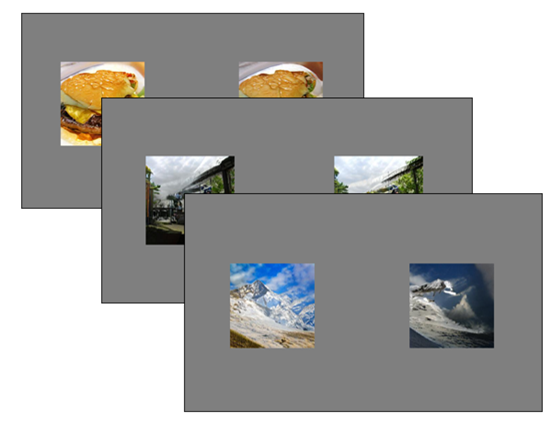
\includegraphics[scale=0.60]{trial_sequence}
	\end{center}
	\vfill
	{\normalfont \textit{Note.} Image depicting three typical trials in the experiment. For every trial, one of the two presented images will be the neutral image with $\alpha=0$, while the other will have an $\alpha$ ranging from $-0.25$ to $0.25$.}
\end{figure}

The experiment was created in JavaScript with the \texttt{jsPsych} library \parencite{de2015jspsych} for its lightweight implementation in browsers, ensuring we have consistent performance independent of the hardware our diverse participant population may have. Each trial consisted of two images generated from the same ImageNet category. One of the two images was always the base image with $\alpha = 0$ while the comparison image was, according to GANalyze at least, either more aesthetic ($\alpha > 0$) or less aesthetic ($\alpha < 0$). The $\alpha$-value for the comparison image differed for each trial, leading to differences in similarity between the base and comparison images for each trial. An $\alpha$-value close to zero indicates high similarity and, consequently, difficulty to discriminate between the images. An $\alpha$-value much larger or smaller than zero indicates low similarity and therefore easy discrimination. The position of the base and comparison image was randomized for each trial to prevent possible confounding factors. There was no time limit for the trials and each stimulus pair stayed on the screen until a participant responded. Each 10-minute block was created to contain a roughly uniform distribution of chosen $\alpha$-values and ImageNet categories to ensure that each participant is presented with a comparable stimulus set. Furthermore, the same ImageNet category never appeared more than once in a block, meaning that the maximum length for a block was 489 trials: the total number of ImageNet categories used.

As this was a relatively fast-paced and demanding task, we added a short break after 5 minutes to counteract fatigue and loss of concentration. After 10 minutes, the task automatically turned to a screen thanking the participants for their assistance and instructing them to click the link that appeared. Clicking this link redirected them to Prolific where their successful participation was registered. They were later given a monetary compensation of £1.38 converted to their local currency, only if they had completed the task seriously, thus providing no irrational data. Our criteria for proper task performance are explained below.



\subsection{Data Analysis}
	\subsubsection{Structural Equation Modeling}
	Our structural model needed to have a latent variable measuring aesthetic experience which also had to be properly explained by the observed variables. In addition, we wanted to know whether age, sex, and nationality affected this. Furthermore, we were interested in the effects of aesthetic experience, age, sex, and nationality on the outcome variable of the behavioral task measured by the proportion of agreement with the neural network. To test this, we used structural equation modeling (SEM) with the \texttt{lavaan} package \parencite{rosseel2012lavaan} in R version 4.1.0 \parencite{rcoreteamlanguage} to build and evaluate models based on theory that would give an explanation to the data. All models were fitted using a maximum likelihood estimation method and the fits were evaluated with the comparative fit index (CFI), Tucker-Lewis index (TLI), and the root mean square error of approximation (RMSEA).
	
	First of all, we performed a priori CFA to validate whether our shortened version of the AEQ was indeed sufficient in explaining the latent aesthetic experience variable. We used the `emotional', `cultural', `perceptual', `understanding', `flow-proximal', and `flow-experience' scales as indicators for our latent variable. 
	
	Next, we moved on to more complicated structural models to better describe the full dataset. More specifically, we created a multiple indicators multiple causes (MIMIC) model aimed to show whether age, sex, and nationality affected the latent aesthetic experience variable. Crucially, we were interested in the effects of the aesthetic experience latent variable and age, sex, and nationality on the outcome of the image comparison behavioral task. We used the proportion of agreement with the GAN as the measure for aesthetic judgement here. Our initial idea for this model consisted of the latent variable, explained by the indicators, affecting aesthetic judgement in the behavioral task. Age, sex and nationality would have an effect on both the latent variable and the behavioral outcome of judgement. We also made another alternative model based on different theoretical arguments. For this second model, we decided that it did not make sense for nationality to have a direct effect on aesthetic judgement, so we removed that effect and instead added an effect of nationality on the cultural scale from the AEQ, as we believed this would make sense. These models would additionally test the questions \textcite{wanzerExperiencingFlowViewing2020} had regarding their homogeneous population sample. 
	
	Even though the new MIMIC model did not appear to be significantly better or worse than the older one, we decided to keep the newer model as it made more sense from a theoretical point of view.
	
	
	
	\subsubsection{Behavioral Experiment}
	We analyzed the results from the behavioral task using a variety of methods. First of all, we cleaned the data by removing participants that had a bias for the left/right stimulus $>25\%$ ($n=2$), performed too close to chance (i.e., $<55\%$ agreement for all $\alpha$-values; $n=9$), responded too fast to reasonably perceive and judge the stimuli (i.e., median RT $<500$ ms; $n=6$), and had an exceptionally low number of trials during the 10-minute experiment (i.e., number of trials $<50$; $n=4$).
	
	To see whether the different $\alpha$-values indeed represent a gradual change in stimulus difference, we fitted the results of all participants aggregated over $\alpha$-levels with a psychometric function using the \texttt{quickpsy} package \parencite{linares2016quickpsy}. We specified the guess rate and lapse rate of this function as free parameters because we believe aesthetic judgement to contain a significant subjective component and therefore considered it unreasonable for participants to agree completely with the network for any $\alpha$-level. Analysis on differences between positive and negative $\alpha$-values was done with polynomial regressions. Finally, we tested for potential confounding factors using a simple two-way analysis of variance (ANOVA).
	
	
	
	\subsubsection{GANalyze Parameters}
	To visualize what makes an image beautiful, we analyzed the image features of the generated images. This is a unique application GANs offer to cognitive science, allowing for substantial control over stimuli that are typically hard to obtain without sacrificing ecological validity \parencite{goetschalckx2021generative}. Using the \texttt{Pillow} library \parencite{clark2015pillow} in Python, we summarized each of the 7,335 images into a single value for various image features. Based on the paper by \textcite{ke2006design}, we decided to compare the mean brightness, contrast, sharpness, and saturation of all images aggregated over their $\alpha$-values, allowing us to track the evolution of these features as the aesthetic value of their corresponding images increases. To measure brightness, we computed the mean pixel values of all images converted to grayscale, resulting in a high and low values for bright and dark images respectively. For contrast, we computed the standard deviation of the pixel values in all grayscale images, resulting in high values for high contrasts, and low values for low contrasts. Sharpness was computed by taking the mean value of the grayscale images transformed with 3x3 Laplacian edge-detection filter. Finally, we measured the saturation by first converting the images from RGB to HSV and then taking the mean value of only the resulting saturation channel. We standardized and centered all resulting values using z-transformations.
		
	In addition, we investigated how the color distributions change as the aesthetic value of the images increases. We did this by plotting histograms for the individual RGB-values of separate images in an image sequence defined by the ImageNet category. We did this for five random image sequences separately rather than averaging over all images for different $\alpha$-levels. Each image sequence is made up of a unique color composition that may affect its aesthetic value in different ways. Averaging over all images for a given $\alpha$-level would then obscure the valuable information that the evolution of single image sequence could offer.
	
	As we have not developed a method to formally investigate high-level image features in this study, we simply looked at the resulting image sequences to find out what changes as the aesthetic value increases. We did not draw any conclusions from this method due to its subjective nature. We did however use our findings here to contextualize the low-level features we found.

\end{document}
